\documentclass[12pt]{article}
\usepackage{fontspec}
\usepackage{polyglossia}
\setmainlanguage{french}
\usepackage{csquotes}
\usepackage{lipsum}

\usepackage{graphicx}% insérer des images
\usepackage{lscape}% mettre en format paysage
\usepackage{subcaption}% plusieurs images côte à côte : environnement subfigure
\usepackage{hyperref}% écrire une adresse web : \url{...}
\hypersetup{hidelinks}% liens cliquables, sans cadre de couleur

% L'image est dans le dossier exercices : on indique à LaTeX où la chercher.
% (Si l'image est dans le même dossier que le fichier .tex, cette ligne est inutile.)
\graphicspath{{../exercices/}}

\begin{document}

\section{Insérer une image}

\lipsum[1]

% 1. 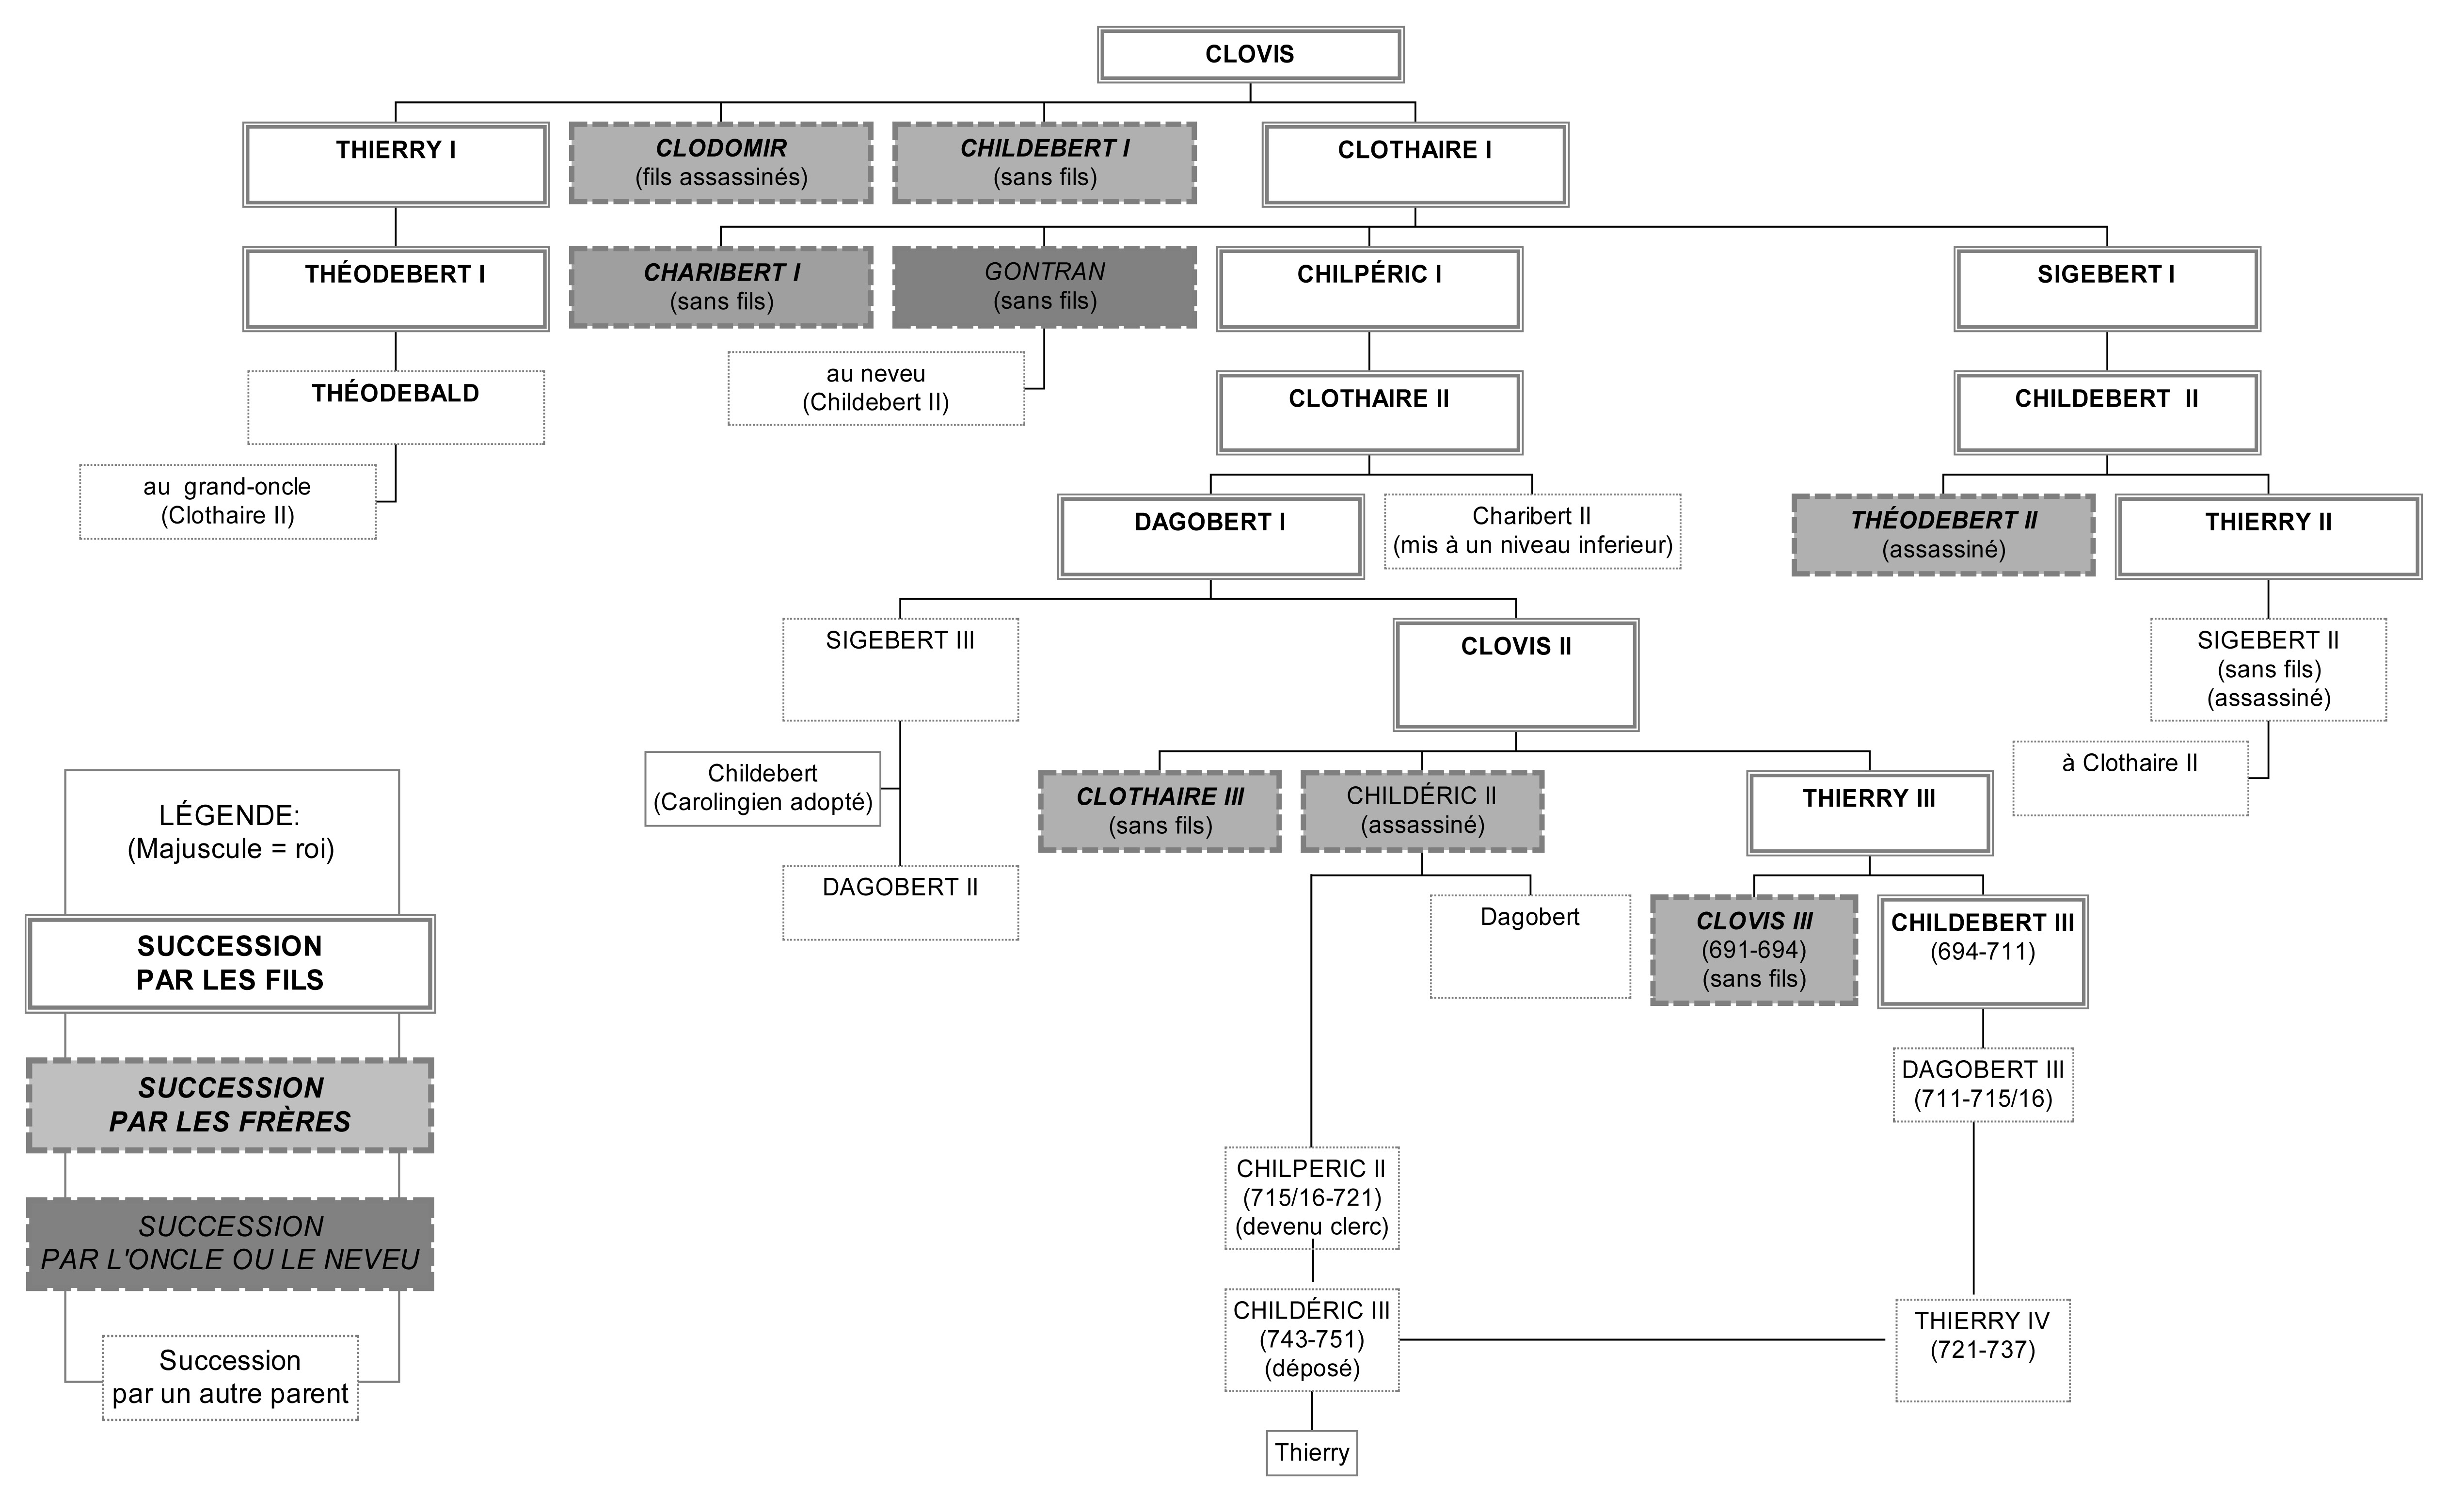
\includegraphics{genealogie.jpg} seul : l'image (5050 × 3119 pixels) est bien trop grande et sort de la page.
% 2. width=\textwidth : l'image prend toute la largeur du texte ; scale=0.1 fonctionne aussi,
%    mais width= est plus sûr, car il ne dépend pas de la taille d'origine de l'image.
% 3. Environnement figure : l'image devient un flottant. [ht] : ici si possible, sinon en haut d'une page.
%    Avec [b], l'image part en bas de page ; avec [p], sur une page à part.
% 4. \caption : légende numérotée. L'argument optionnel (entre crochets) est la version courte,
%    utilisée dans la liste des figures (sans l'adresse de la source).

\begin{figure}[ht]
	\centering
	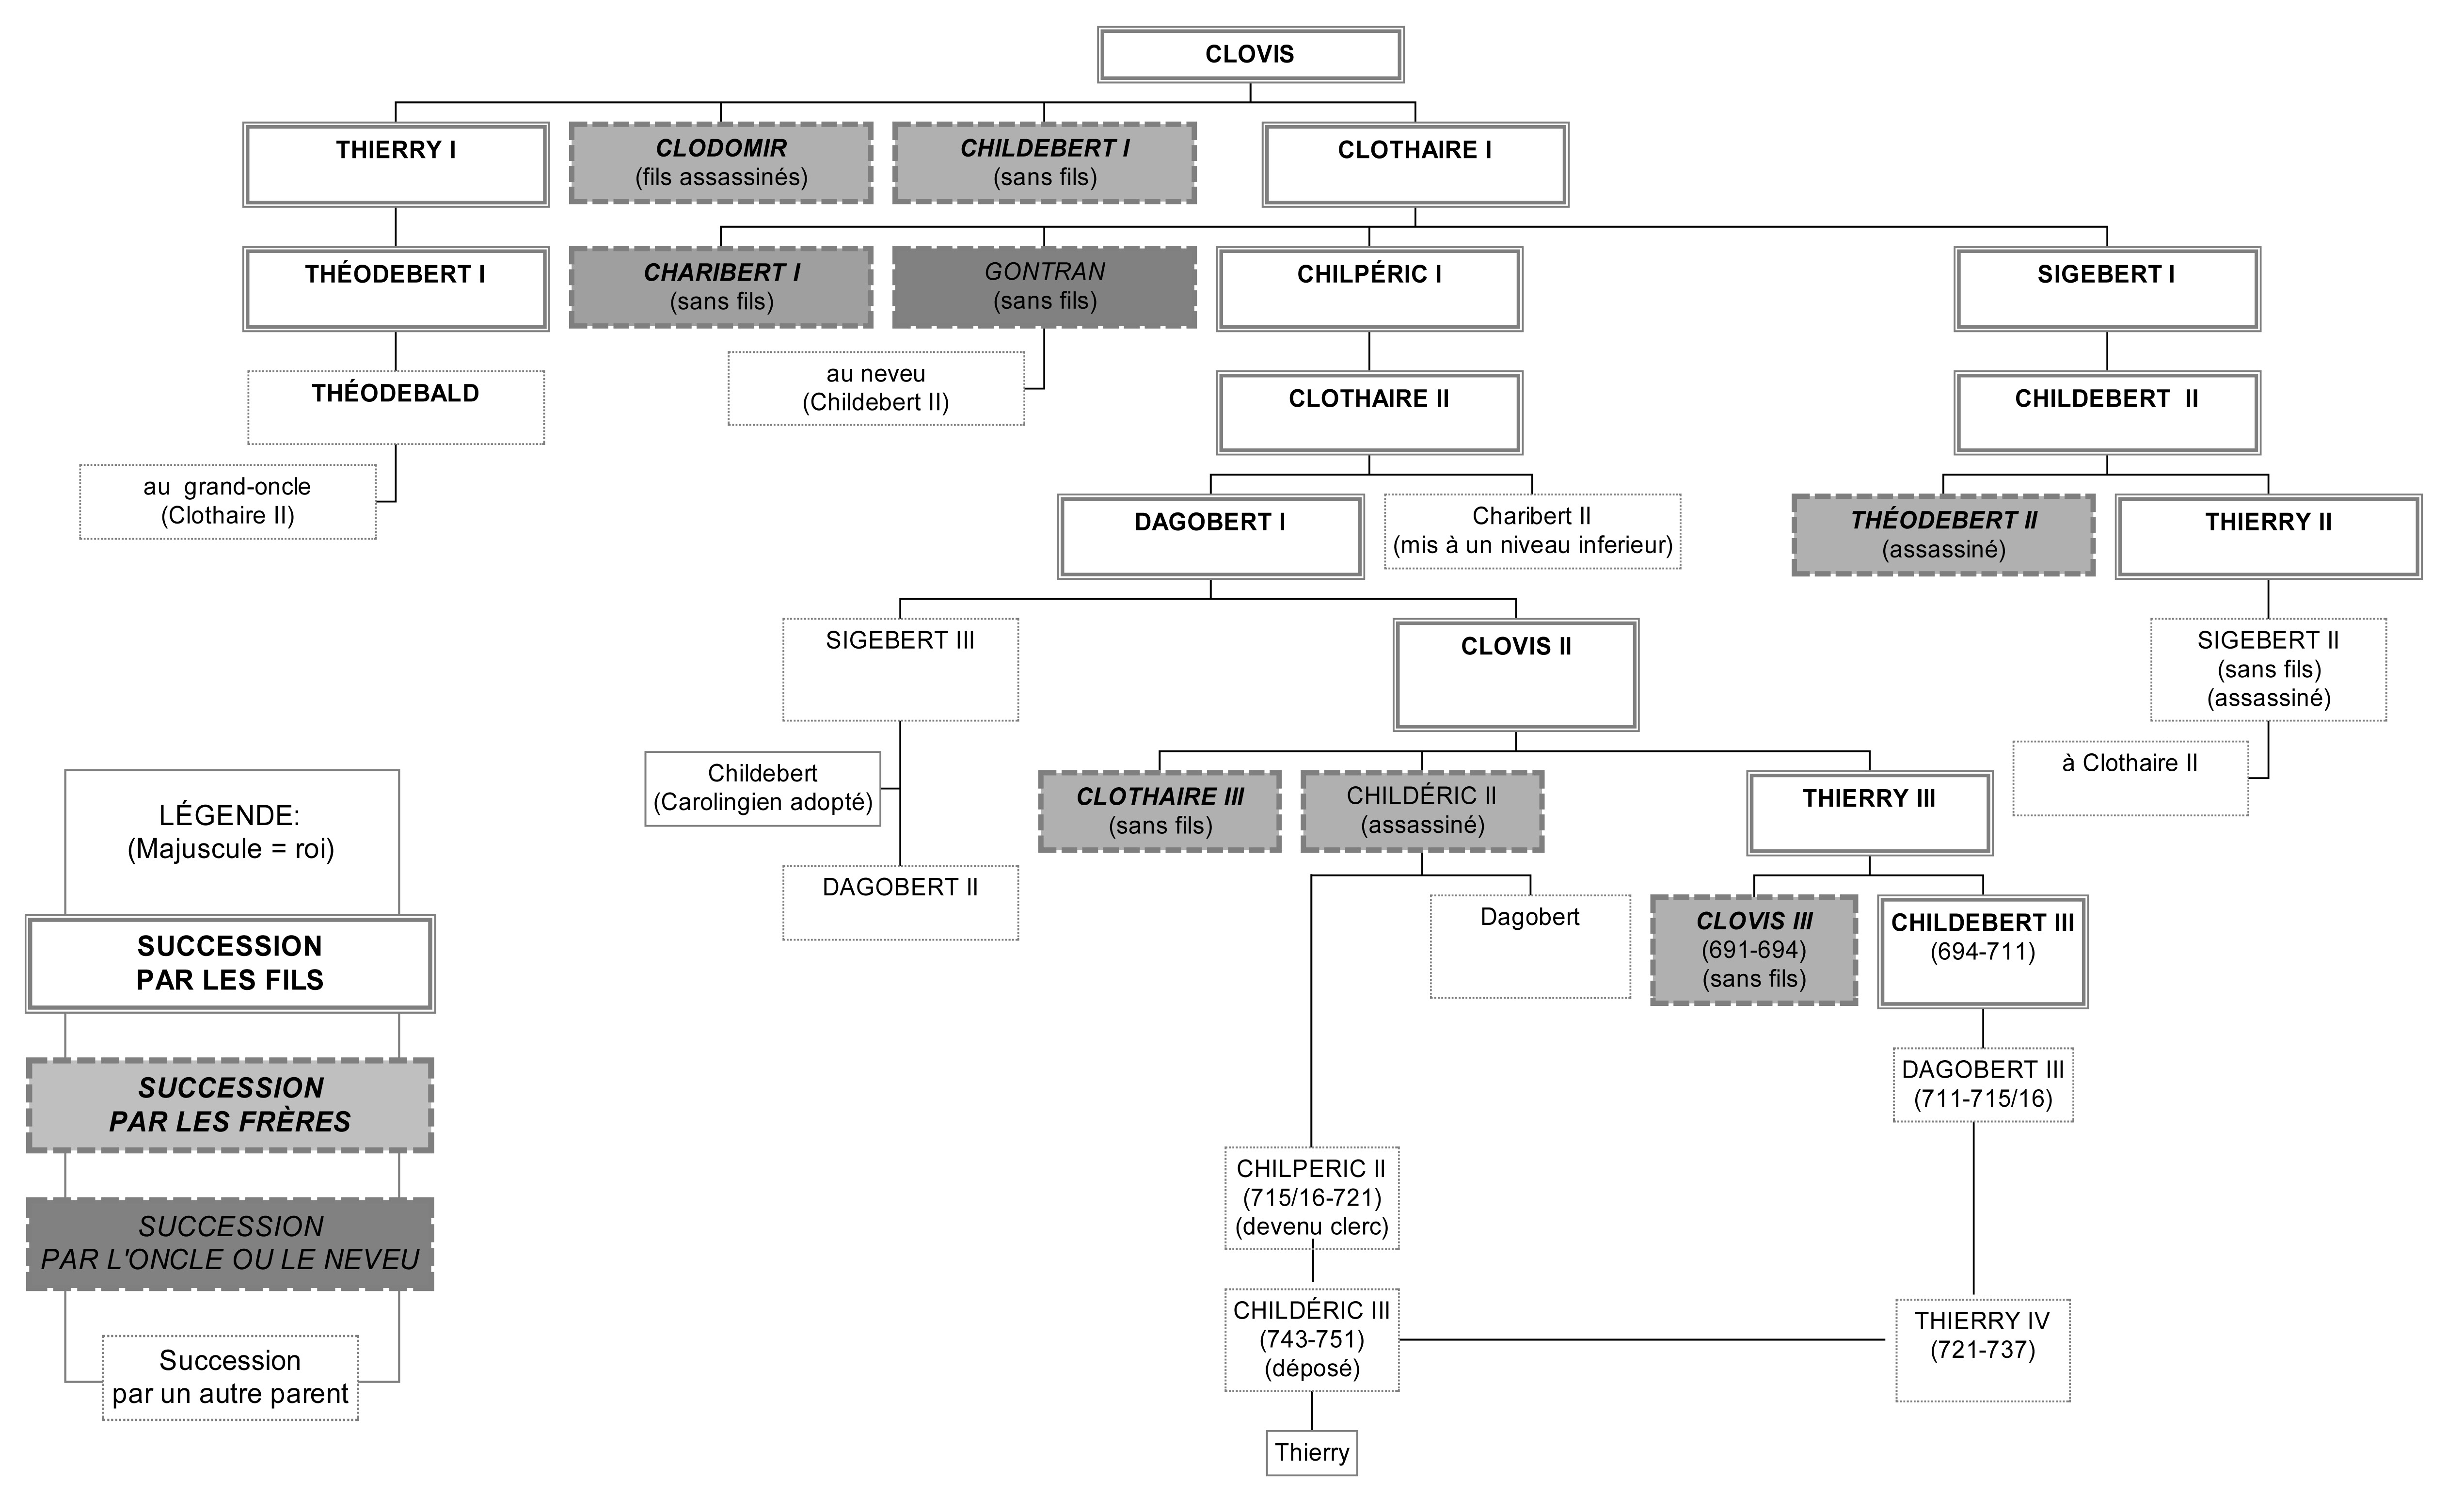
\includegraphics[width=\textwidth]{genealogie.jpg}
	\caption[Arbre généalogique]{Arbre généalogique. Source : \url{https://books.openedition.org/efr/2282}}
\end{figure}

\lipsum[2]

% 5. Format paysage : l'environnement landscape fait tourner la page entière.
%    Sans réglage de taille l'image déborde encore : on la règle sur la largeur de la page tournée (\linewidth).
%    landscape commence toujours une nouvelle page.

\begin{landscape}
	\begin{figure}
		\centering
		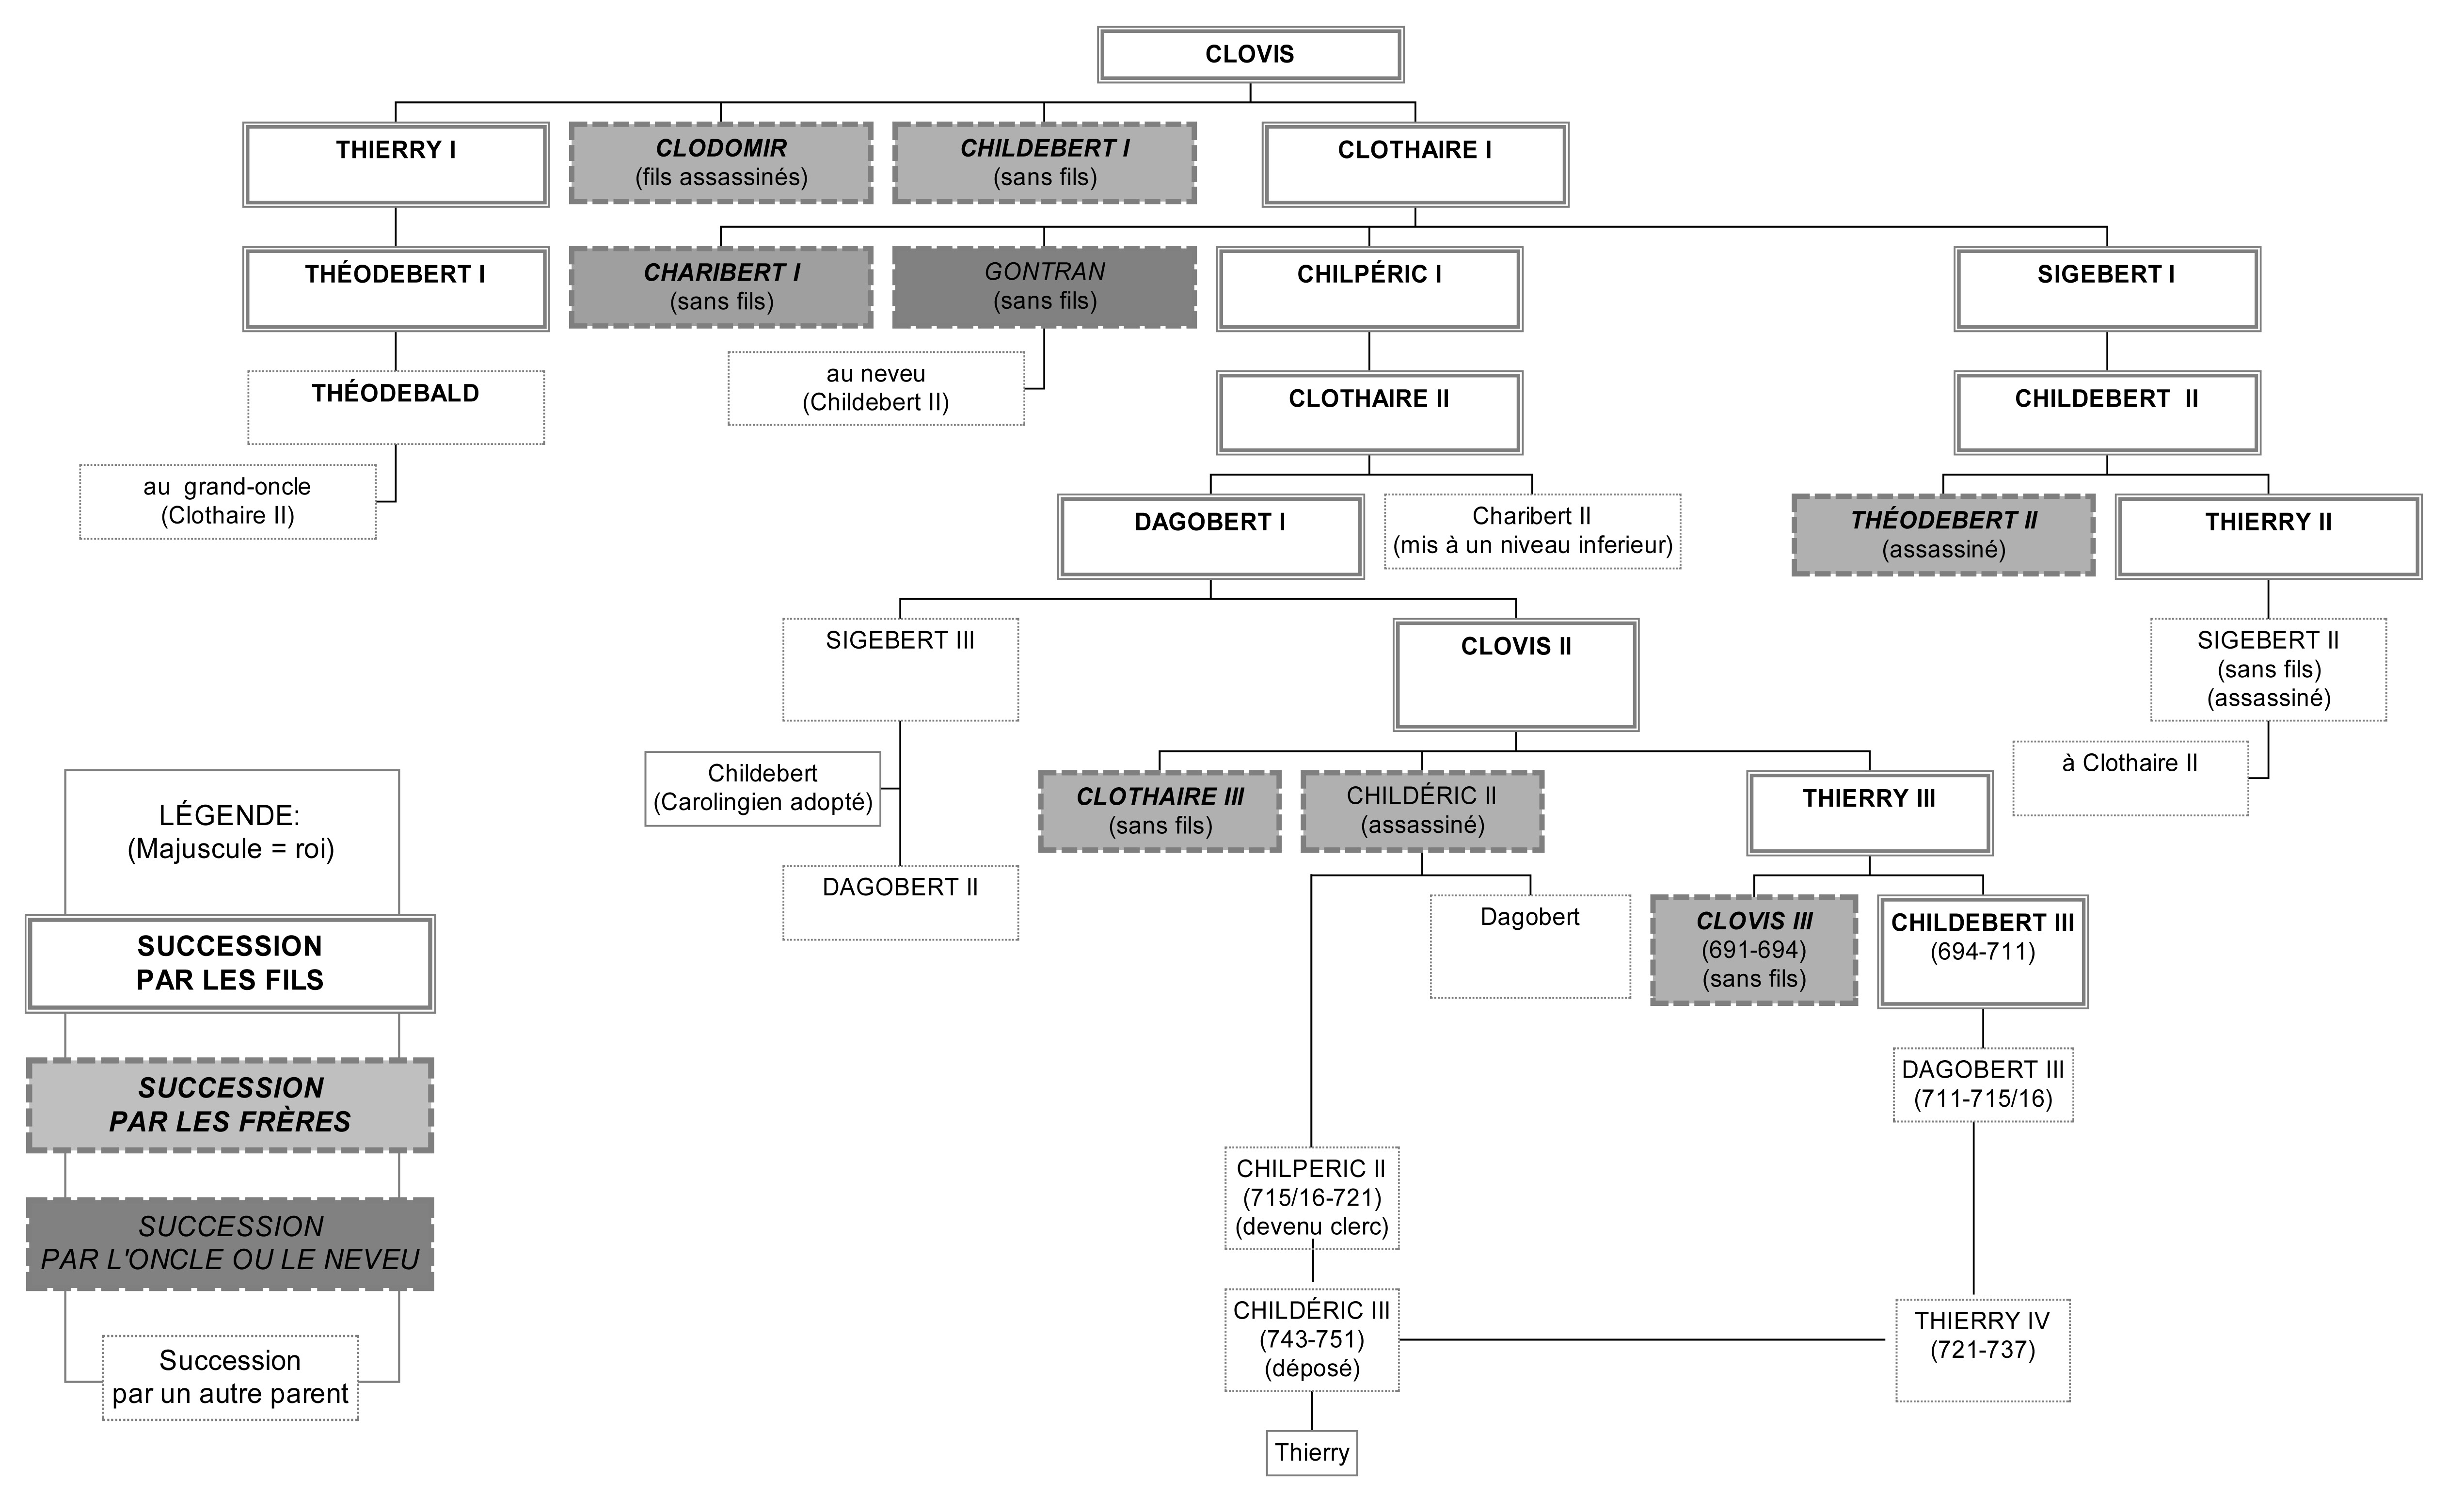
\includegraphics[width=\linewidth]{genealogie.jpg}
		\caption[Arbre généalogique (paysage)]{Arbre généalogique, en format paysage. Source : \url{https://books.openedition.org/efr/2282}}
	\end{figure}
\end{landscape}

\lipsum[3]

% 6. Un seul flottant figure, qui contient une subfigure par image.
%    {.45\textwidth} : largeur de chaque subfigure ; les deux font moins que \textwidth.
%    width=\linewidth : l'image prend toute la largeur de sa subfigure.
%    \hfill repousse les deux images vers les bords, l'espace restant va au milieu.
%    Chaque \caption d'une subfigure donne (a), (b) ; le dernier \caption est la légende commune.
%    Une ligne blanche entre les deux subfigure crée un nouveau paragraphe : les images passent l'une sous l'autre.

\begin{figure}[ht]
	\centering
	\begin{subfigure}{.45\textwidth}
		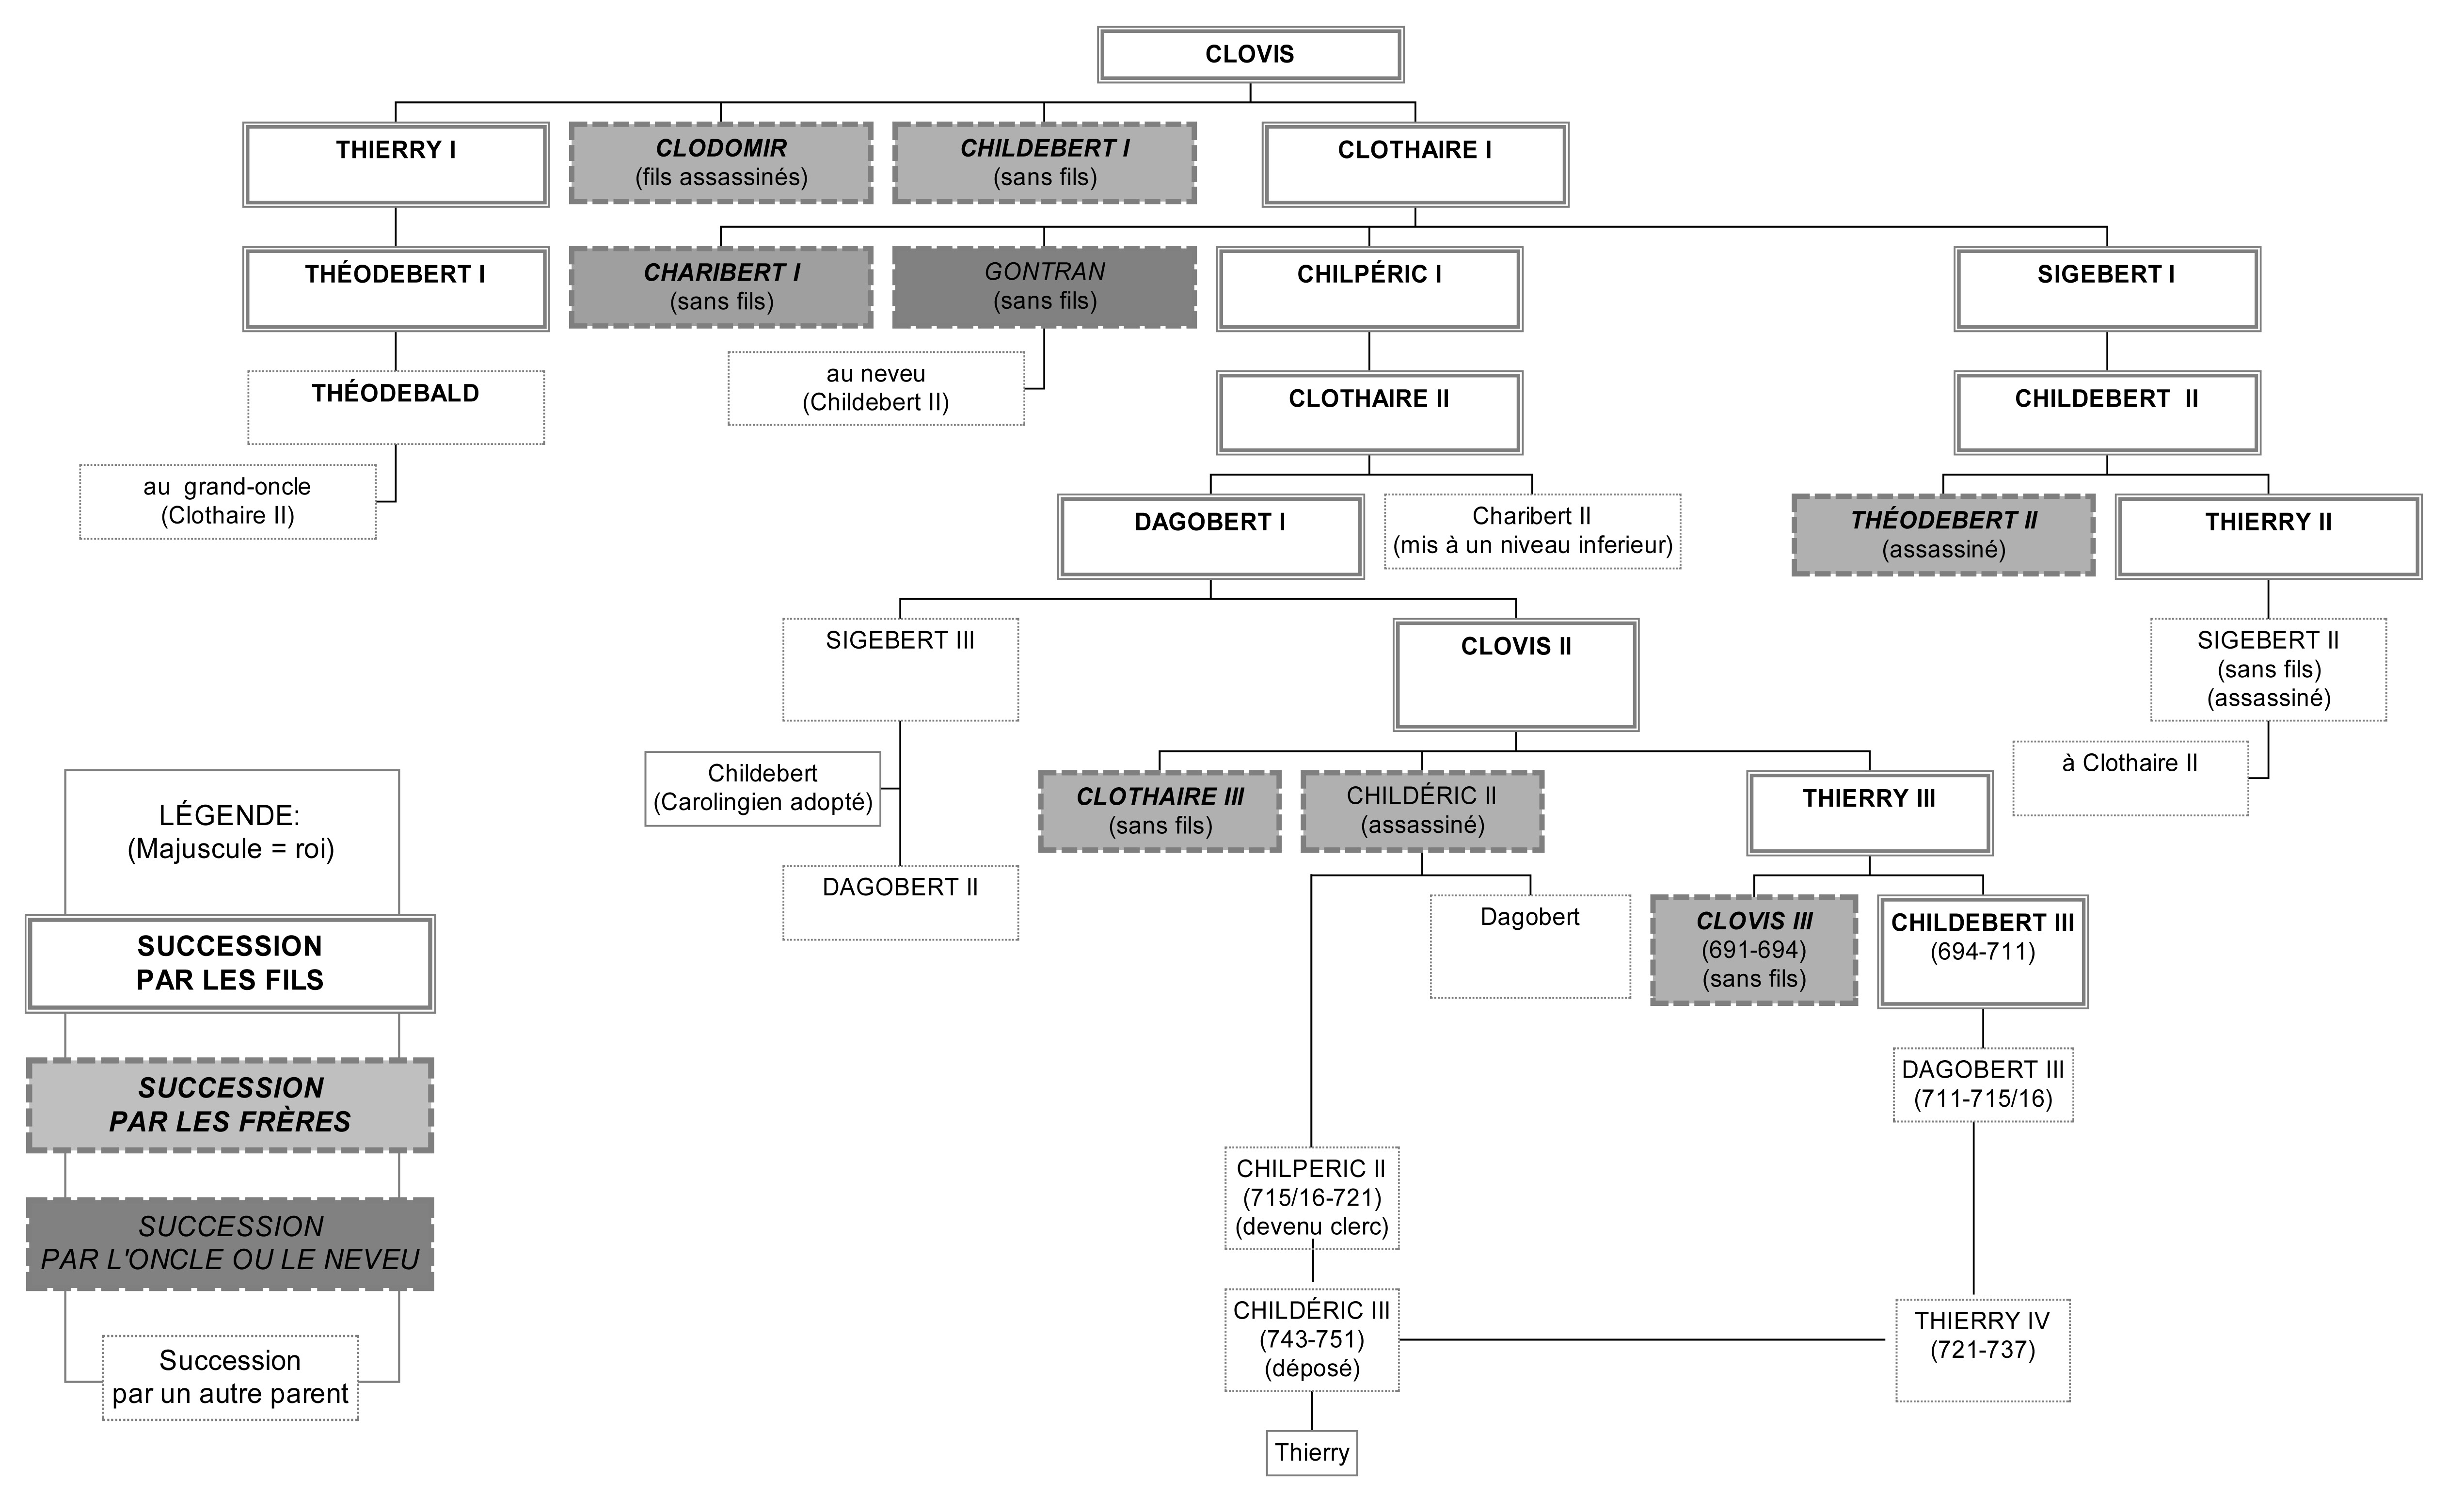
\includegraphics[width=\linewidth]{genealogie.jpg}
		\caption{Première version}
	\end{subfigure}
	\hfill
	\begin{subfigure}{.45\textwidth}
		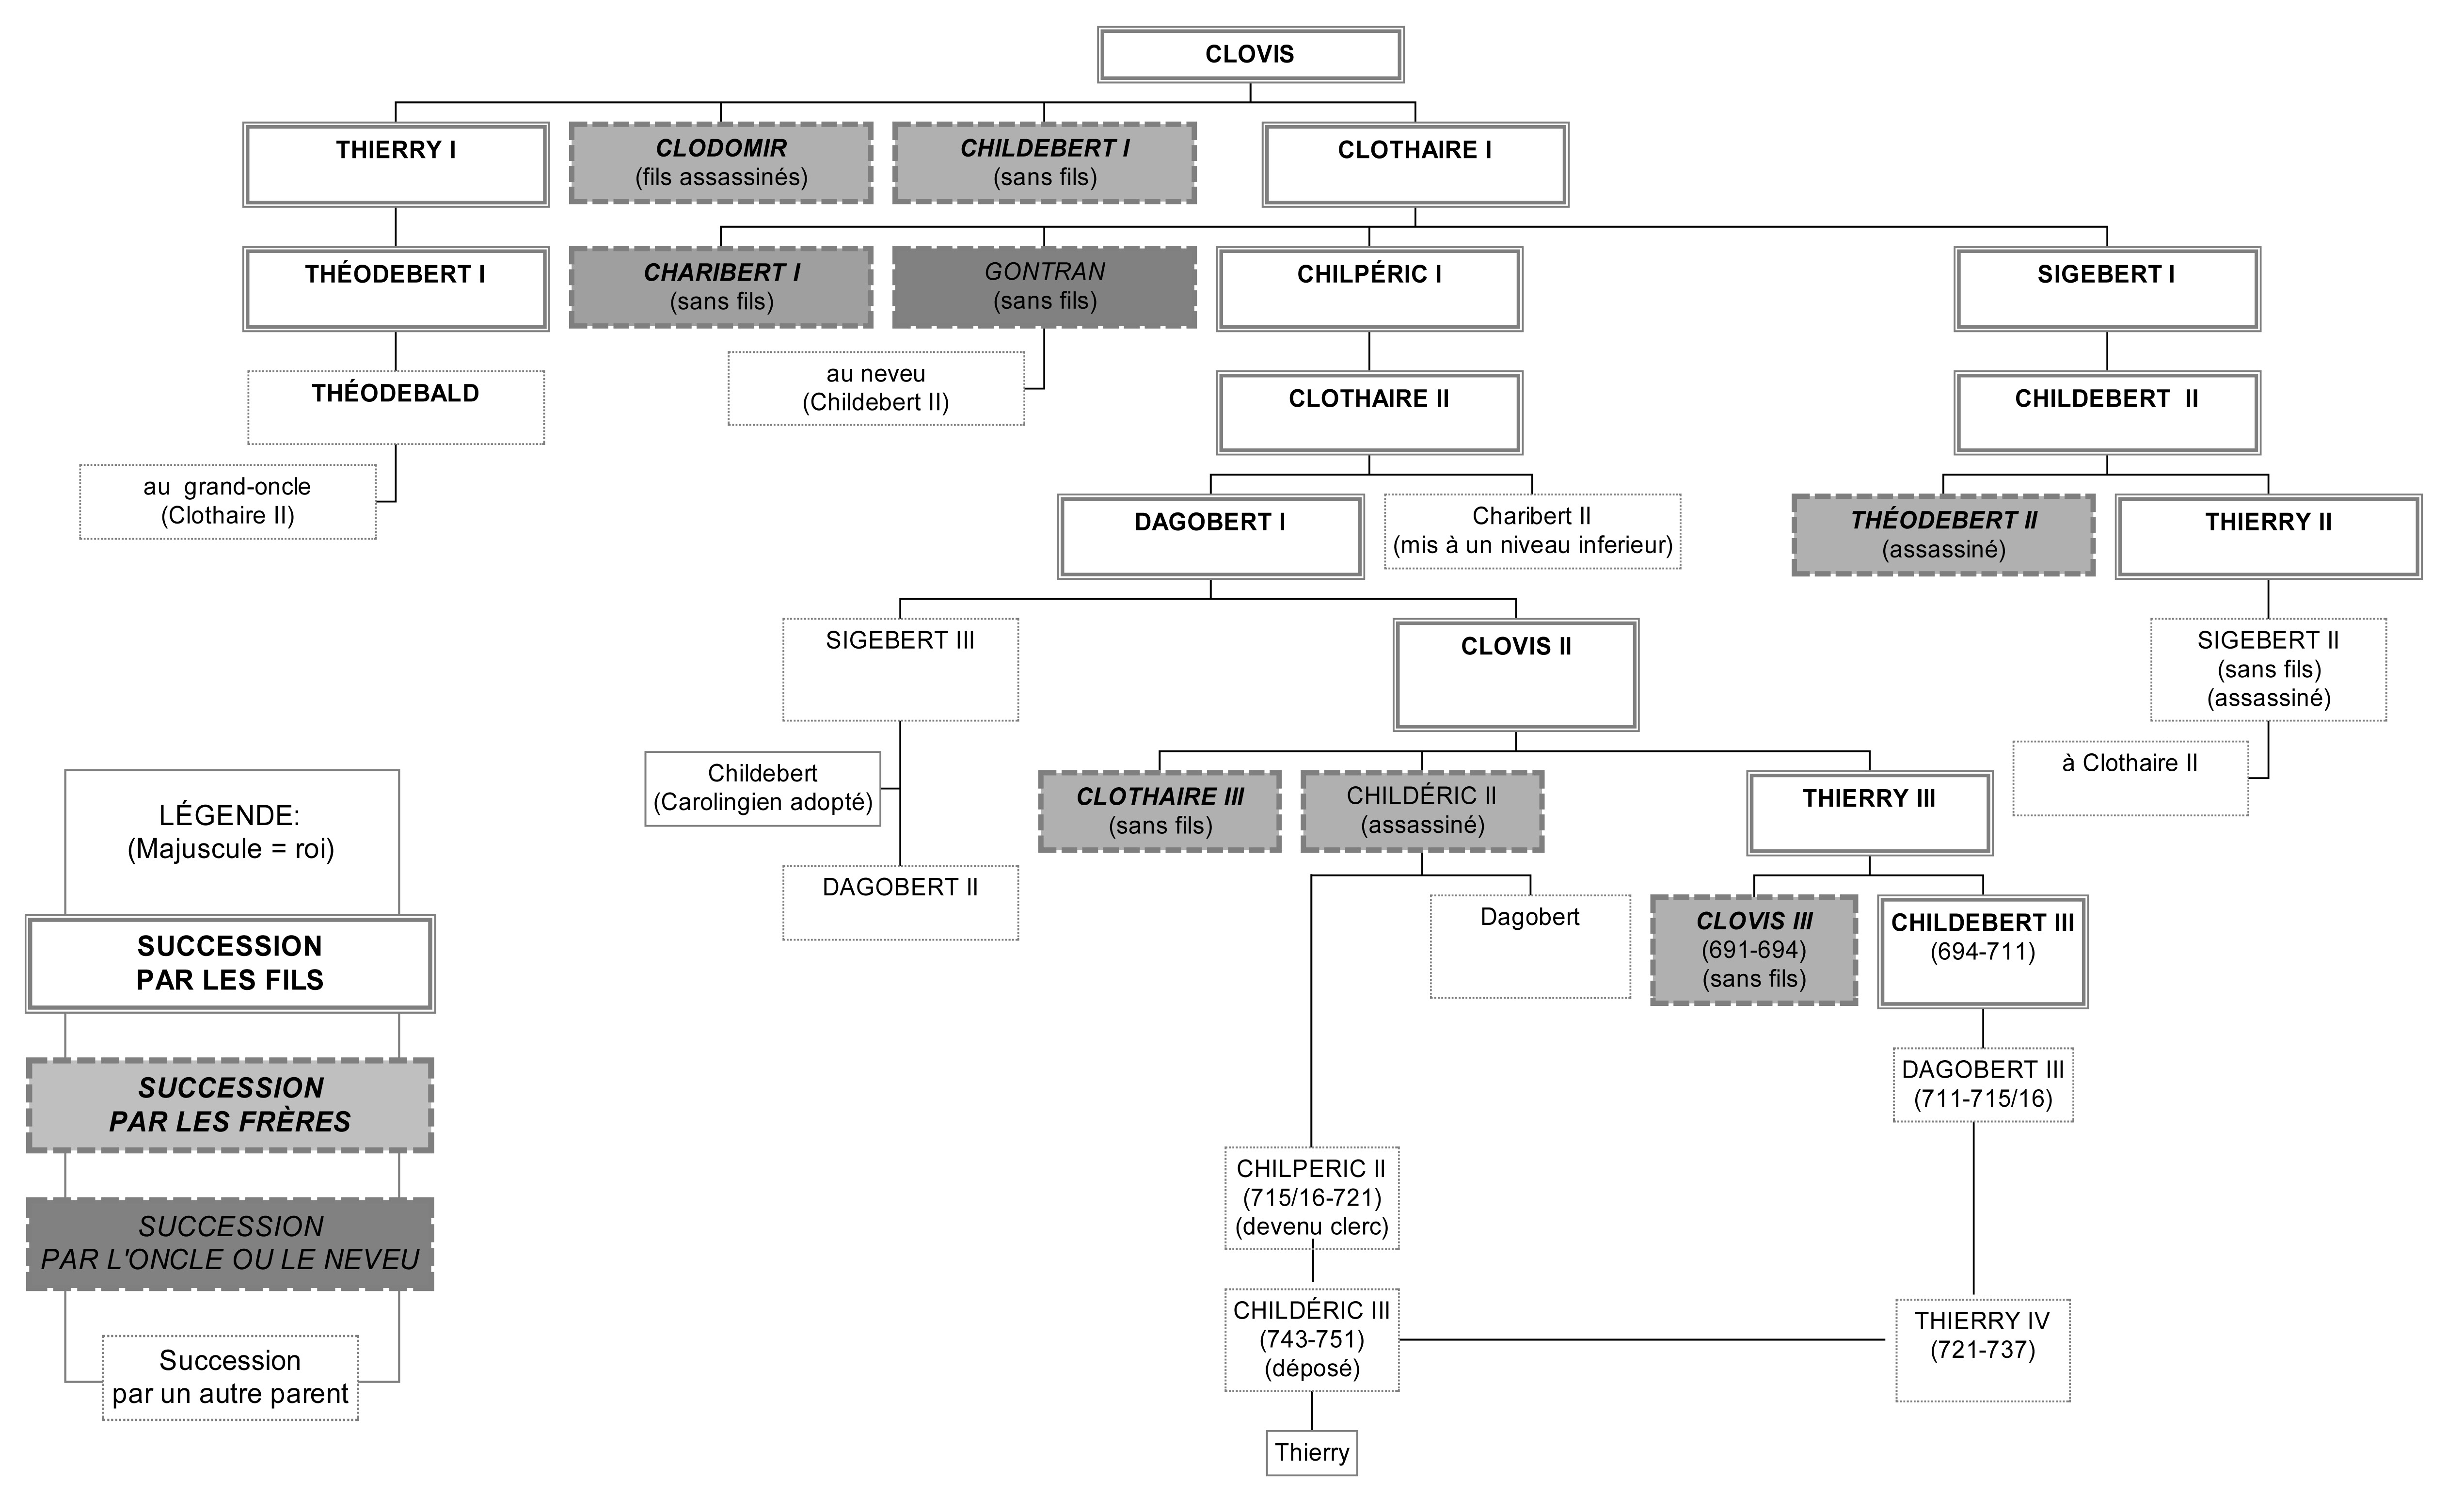
\includegraphics[width=\linewidth]{genealogie.jpg}
		\caption{Seconde version}
	\end{subfigure}
	\caption[Deux images côte à côte]{Deux images côte à côte. Source : \url{https://books.openedition.org/efr/2282}}
\end{figure}

\lipsum[4]

% 7. Liste des figures (deux compilations sont nécessaires pour qu'elle apparaisse).
\listoffigures

\end{document}
